\section{Software Diversification}
\label{sota:sota}
%Checkmarck symbol
\def\checkmark{\tikz\fill[scale=0.4](0,.35) -- (.25,0) -- (1,.7) -- (.25,.15) -- cycle;} 

% Commands to refer to the milestones
\newtheoremstyle{sota}% name of the style to be used
  {\topsep}% measure of space to leave above the theorem. E.g.: 3pt
  {\topsep}% measure of space to leave below the theorem. E.g.: 3pt
  {\itshape}% name of font to use in the body of the theorem
  {0pt}% measure of space to indent
  {\bfseries}% name of head font
  {}% punctuation between head and body
  { }% space after theorem head; " " = normal interword space
  {(\thmname{#1}\thmnumber{#2})\textnormal{\thmnote{ (#3)}}}

\def\Gnospace~{G{}}
\theoremstyle{sota}
\newtheorem{goal}{G}
\providecommand*{\definitionautorefname}{\Gnospace}
\newcommand{\goalautorefname}{\Gnospace}


\def\Snospace~{S{}}
\theoremstyle{sota}
\newtheorem{strategy}{S}
\providecommand*{\definitionautorefname}{\Snospace}
\newcommand{\strategyautorefname}{\Snospace}

\def\Unospace~{U{}}
\theoremstyle{sota}
\newtheorem{usage}{U}
\providecommand*{\definitionautorefname}{\Unospace}
\newcommand{\usageautorefname}{\Unospace}

%\%todo{Esta muy regado ahora.}

%\todo{Stress input-output equivalence in the artificial diversification.}

%\todo{Mention concrete objective and achievement when citing.}

%\todo{emove some strategies, just cite some papers and thats it. Reduce to five transformations. Stick to U2 andd U3. Add techincal stack in the table.}

%\todo{Add level of transformation as a dimension. Hoigh level, fine-grained transofmrations, etc}

%\todo{Start with COhen, then go form high level to fine granied and from technologies to LLVM and Wasm.}


%\todo{Given a collection of pgorams, then enumerate the usages. Second approach, multiple encapsulation in one single program.}

Software Diversification has been widely studied in the past decades. This section discusses its state of the art.
% What is Software diversity
Software diversification consists in synthesizing, reusing, distributing, and executing different, functionally equivalent programs. 
According to the survey of Baudry and Monperrus \cite{natural_diversity}, the motivation for software diversification can be separated in five categories: reusability \cite{pohl2005software}, software testing \cite{Chen2010AdaptiveRT}, performance \cite{10.1145/2025113.2025133}, fault tolerance \cite{1659219} and security \cite{cohen1993operating}. Our work contributes to the latter two categories. In this section we discuss related works by highlighting how they generate diversification and how they use the generated diversification. We finalize by comparing our contributions with the related work.

\subsection*{Artificial Software Diversity.}

There are two primary sources of software diversification: Natural and Artificial Diversity \cite{natural_diversity}. This work contributes to the state of the art of Artificial Diversity, which consists of artificially synthesizing software. 
% Intro to Cohen and that functional/semantic equivalence is 
We have found that the foundation for automatic software diversity has barely changed since Cohen in 1993 \cite{cohen1993operating}. Therefore, the work of Cohen is the cornerstone of this dissertation.
According to their seminal work, whatever two programs are equal if they are semantically equivalent, thus, one program can be considered a diversified version of the other. 
They defined semantic/functional equivalence as input-output equivalence. Two programs are equivalent if, given identical input, they produce the identical output. 

% Mutation strategy
Cohen \etal proposed to generate automatic software diversification through mutation strategies.
A mutation strategy is a set of rules to define how a specific component of software development should be changed to provide a different yet functionally equivalent program. Cohen \etal proposed 10 concrete transformation strategies that we summarize, complemented with the work of Baudry and Monperrus \cite{natural_diversity} and the work of Jackson \etal \cite{jackson}, in 5 strategies.

% A mutation can be applied at different layers of software lifecycle, from compilation to execution and from source code to executable binary.


%Natural diversity can be controlled or an unpredicted consequence of developing processes. Controlled natural diversity is usually called Design Diversity or N-Version Diversity. It is addressed using engineering decisions \cite{1659219}. 
%In practice, Natural Diversity consists of providing N development teams with the exact requirements. The teams develop N independent versions using different approaches. On the other hand, Natural Diversity can emerge from spontaneous software development processes. To illustrate the Natural Diversity phenomenon, CodeForces\footnote{\url{https://codeforces.com/contest/1667/status/page/2?order=BY_PROGRAM_LENGTH_ASC}} shows more than 350 different and successful solutions in C++ for a single requirements based problem in a single programming contest. 
%The software market is an expected source of natural diversity. Sengupta \etal \cite{10.5555/3091125.3091155} used this fact to reach the security goal (\autoref{goal:security}).



% Jump to the need of artificial
%Notice that Natural Diversity can rely on itself to escalate, and it is coped by the preexistence of software. This might be a limitation. For example, in the context o this work, the natural diversity for \wasm programs is nearly inexistence \cite{Hilbig2021AnES}. When natural diversity is not enough, it is innate to think that the source for diversification needs to be artificial. 

% Classification by Cohen



\begin{strategy}{Equivalent instructions replacement}
    \label{strategy:S1}
    \normalfont 
    Pieces of programs can be replaced by semantically equivalent code such as equivalent arithmetic expressions, including the adding of garbage instructions, \ie instructions that do not affect the computation result. This strategy is simple but powerful since the complexity of program variants dramatically increases. In terms of overhead, the size of the program variant increases with the size of the replacement. Usually, the replacement rules are written by hand as code templates representing a piece of code and a valid replacement for it, similar to compiler optimization rules. For example, Jackson \etal \cite{jackson2011compiler} highlighted the usage of  the optimization flags of several compilers to generate semantically equivalent binaries. On the same topic, Cleemput \etal \cite{Cleemput2012} and Homescu \etal~\cite{homescu2013profile} introduce the usage of inserting NOP instructions to generate statically different variants at each compilation. 


    %Jackson \etal \cite{jackson} have explored how to use NOP operations inserted during compiling time to diversify programs \todo{which stack, if LLVM merge with the previous one}. 
    % However, this approach is limited by the number of available flags in the compiler implementation and because the optimization is applied in all possible places in the code at the same time.
    Exhaustive exploration is another approach to generate equivalent instructions. This technique is based on sampling or constructing all possible programs for a specific language. Once a program is found, it is checked for semantically equivalence against the original program, reporting it as a variant if is the case.
     Jacob \etal \cite{jacob2008superdiversifier} proposed the technique called superdiversification for x86 binaries. They generate semantically equivalent transformations at basic block level that outperform transformations written by human experts. Similarly, Tsoupidi \etal \cite{Tsoupidi2020ConstraintBasedSD} introduced Diversity by Construction, a constraint-based compiler to generate software diversity for MIPS32 architecture. Their technique relies in using a constraint solver to generate program variants that by construction are semantically equivalent. Compared to other techniques, the works of Jacob \etal and Tsoupidi \etal do not need the writing of transformation strategies by hand, but they are limited by the reach of theorem solvers and can only be applied statically. 
     \\
     \\

    %An enumerative synthesis is a brute-force approach to generate program variants. With a maximum number of instructions, it constructs and checks all possible programs up to that limit. For a simplified instance, with a maximum code size of 2 instructions in a programming language with $L$ possible constructions, an enumerative synthesizer builds and checks all $L\times L$ combinations of programs. 
    %
\end{strategy}


\begin{strategy}{Instruction reordering}
    \label{strategy:S2}
    \normalfont
    This strategy reorders instructions or entire program blocks if they are independent.
    The location of variable declarations might change as well if compilers resort them in the symbol tables. It prevents static examination and analysis of parameters and alters memory locations. The strategy should not affect the size of program variants neither their execution time. For example, Bhatkar \etal \cite{bhatkar03, bhatkar2005efficient} proposed the random permutation of the order of variables and routines for ELF binaries.
\end{strategy}

\begin{strategy}{Adding, changing, removing jumps and calls}
    \label{strategy:S5}
    \normalfont
    This strategy creates program variants by adding, changing, or removing jumps and calls in the original program. Cohen \cite{cohen1993operating} mainly illustrated the case by inserting bogus jumps in programs. Pettis and Hansen \cite{pettisochhansen} proposed to split basic blocks and functions for the PA-RISC architecture, inserting jumps between splits.
    Similarly, Crane \etal~\cite{crane2015thwarting} de-inline basic blocks of code as an LLVM 3.3 pass. In their approach, each de-inlined code is transformed into semantically equivalent functions that are randomly selected at runtime to replace the original code calculation. On the same topic, Bhatkar \etal \cite{bhatkar2005efficient} extended their previous approach \cite{bhatkar03}, replacing function calls by indirect pointer calls in C source code, allowing post binary reordering of function calls.
\end{strategy}


\begin{strategy}{Program memory and stack randomization}
    \label{strategy:S7}
    \normalfont
    This strategy changes the layout of programs in the host memory. Also, it can randomize how a program variant operates its memory. The work of Bhatkar \etal \cite{bhatkar03, bhatkar2005efficient} also proposed to randomize the base addresses of applications and the library memory regions, and the random introduction of gaps between memory objects in ELF binaries. Tadesse Aga and Autin \cite{aga2019smokestack} and Lee \etal \cite{lee2021savior} recently proposed a technique to randomize the local stack organization for function calls using a custom LLVM compiler.
    Younan \etal \cite{Younan2006} proposed to separate a conventional stack into multiple stacks where each stack contains a particular class of
    data. 
    On the same topic, Xu \etal \cite{xu2020merr} transform programs to reduce memory exposure time, improving the time needed for frequent memory address randomization. 
    %This makes it very hard for an attacker to ignore the key to inject executable code. This breaks the predictability of program execution and mitigates certain exploits. 
\end{strategy}


\begin{strategy}{ISA randomization and simulation}
    \label{strategy:S8}
    \normalfont
    This strategy encodes the original program binary, for example, by using a simple XOR operation over its binary bytestream. Once encoded, the program can be decoded only once at the target client, or it can be interpreted in the encoded form using a custom virtual machine implementation. This technique is strong against attacks involving the examination of code. It does not affect the size of program variants or their execution times.
    Kc \etal and Barrantes \etal \cite{Kc03,barrantes2003randomized} proposed seminal works on instruction-set randomization 
    to create a unique mapping between artificial CPU instructions and real ones.
    On the same topic, Chew, and Song \cite{Chew02mitigatingbuffer} target operating system randomization. They randomize the interface between the operating system and the user applications: the system calls, the library entry points (memory addresses), and the stack placement. 
    Courouss{\'e} \etal~\cite{courousse2016runtime} implement an assembly-like DSL to generate equivalent code at runtime in order to increase protection against side-channel attacks. Their technique generates a different program during execution using an interpreter for their DSL.

    %It is an interpretation mechanism similar to encoding (\autoref{strategy:S9}), but the execution of programs is delegated to a custom interpreter instead of using preexisting execution hosts. The program is decoded at runtime every time it is invoked. 
    
\end{strategy}


\begin{comment}

\begin{strategy}{Intermixing}
    \label{strategy:S10}
    \normalfont
    With the existence of more than one program variant, the execution of program variants can be mixed. The decision of which variant executes is decided at runtime. This strategy is the core for randomization, multivariant execution and the execution by consensus defined in \autoref{goal:reliability}. This strategy is 
    complex to implement because the integrity of the memory and stack needs to be stable between programs.
\end{strategy}
\end{comment}

%\subsection*{Vertical Software Diversification}

The mentioned techniques can be applied at any layer of the software lifecycle, at coarse-grained level or fine-grained level.
At high-level, Harrand \etal, propose to merge several Java decompiler variants to provide an extended and improved meta-decompiler \cite{harrand2020java}. On the same topic, Sengupta \etal \cite{10.5555/3091125.3091155} shift several database engines and backends for web applications. Their idea makes known CVEs to be available only in certain time window, making potential attackers to not always success. Moreover, Roi \etal \cite{10.1145/3318216.3363338} proposed to use several machine learning algorithms with the same task to tackle adversarial attackers, using a different algorithm every time the system was queried.
These works used preexisting software diversity to provide improved systems, both for reliability and security.

On the other hand, the before mentioned mutation strategies can be applied directly to the basecode, during the compilation of programs and directly to the generated binaries. As we previously mentioned Homescu \etal \cite{homescu2013profile}, Jackson \etal \todo{jackson}, Jacob \etal \cite{jacob2008superdiversifier}, Crane \etal \cite{crane2015thwarting}, Aga \etal \cite{aga2019smokestack} and Tsoupidi \etal \cite{Tsoupidi2020ConstraintBasedSD} placed compilers in their diversification techniques. Similarly, Bathkar \etal \cite{bhatkar03,bhatkar2005efficient}, Chew and Song \cite{Chew02mitigatingbuffer}, El-Khalil and Keromytis \cite{ElKhalil2004}, and Cohen \cite{cohen1993operating} itself mostly proposed binary to binary transformations. 
We have observed that fine-grained techniques are mainly motivated because they provide more robust diversification in terms of preservation. For example, to apply diversification techniques closer to the final execution avoid removing of code transformations by later optimization or compilation stages. Besides, in terms of implementation, fine-grained diversification can be achieved \todo{Improve}.

%Superdiversifier, all the others, and then finish with that we contribute to fine-grained.

\subsection*{Usages of Software Diversity}

After program variants are generated, they can be used in two main scenarios: Randomization or Multivariant Execution(MVE) \cite{jackson}. In \autoref{diagrams:sota:randomization} and \autoref{diagrams:sota:mve} we illustrate both scenarios. 



\newcommand{\rulesep}{\unskip\ \vrule\ }
\begin{figure}[h]
    \centering
    \begin{subfigure}[t]{0.45\textwidth}
        \centering
        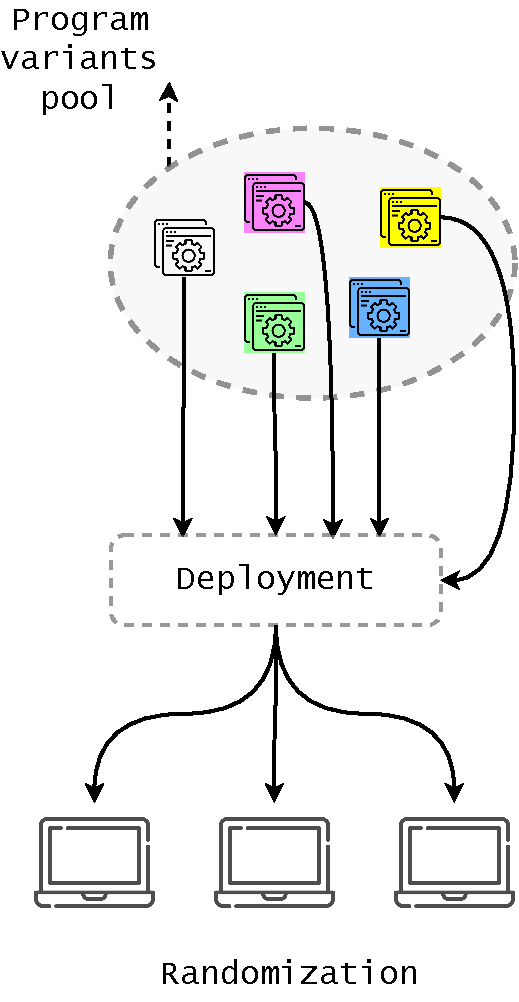
\includegraphics[height=3.1in]{diagrams/randomization.pdf}
        \vspace{0.5cm}
        \caption{Randomization scenario. Given a pool of program variants, one variant is deployed per host. Each deployment randomly selects which variant is assigned to each host. The same program variant is executed in the host at every program invocation between deployments. }        \label{diagrams:sota:randomization}

    \end{subfigure}
    \hspace{1.5mm}
    \rulesep
    \hspace{1.5mm}
    \begin{subfigure}[t]{0.45\textwidth}
        \centering
        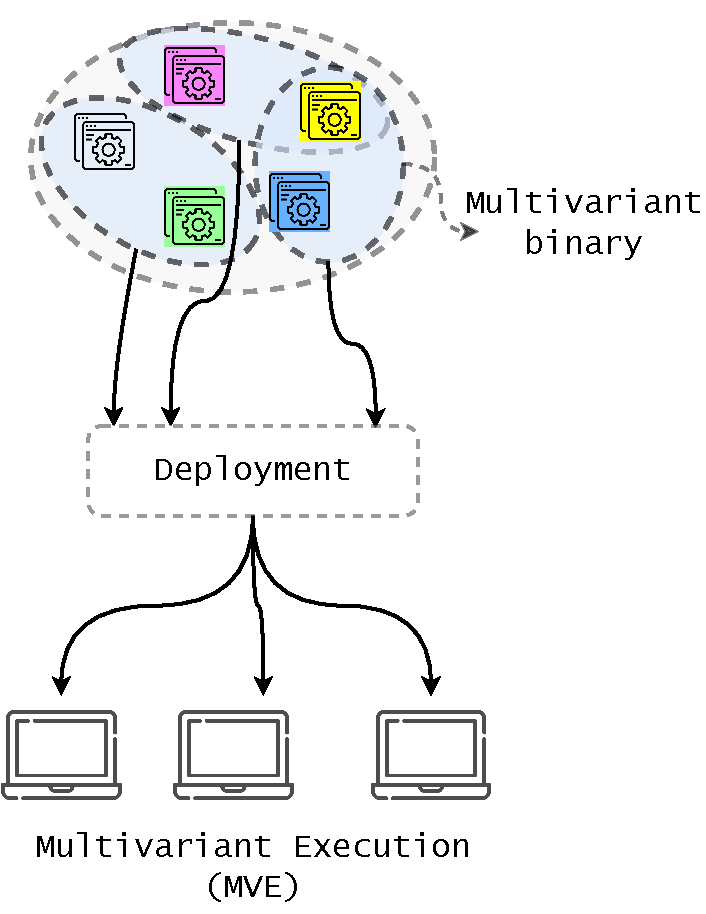
\includegraphics[height=2.8in]{diagrams/mve.pdf}
        \caption{Multivariant Execution scenario. Given a pool of program variants, a sample of the pool is packaged in a multivariant binary that is deployed per. Each deployment randomly selects which multivariant binary is assigned to each host. A variant from the multivariant binary is randomly executed at runtime in the host, .}        \label{diagrams:sota:mve}

    \end{subfigure}
    \caption{Software Diversification usages. }
\end{figure}



\begin{usage}{Randomization:}
    \label{usage:randomization}
    \normalfont
    In the first scenario, a program is selected from the collection of variants (program's variant pool) and at each deployment it is assigned to a random client. This strategy prevents the usage of one variant to exploit another clients. When clients run two program variants, a potential attacker must create one attack for each variant. Therefore, the attacker must spend more time and effort to get the same return on reward for an attack. Jackson \etal \cite{jackson} call this a herd inmunity.

    To illustrate the impact of this idea, the Polyverse company \footnote{\url{https://polyverse.com/}} is able to provide unique Linux distributions to each one of their clients. 

    
    
\end{usage}

\begin{usage}{Multivariant Execution(MVE):}
    \label{usage:mve}
    \normalfont
    In the second scenario, multiple program variants are composed in one single binary (multivariant binary) that is randomly deployed to a client. Once in the client, the multivariant binary executes program variants during runtime, either in parallel to check for inconsistencies or a single program to randomize execution paths \cite{bhatkar03}. Bruschi et al. \cite{bruschi2007diversified} and Salamat et al. \cite{salamat2007stopping} pioneered the idea of executing the variants in parallel. They created a C compiler and modified a standard library that generates 32-bit Intel variants where the stack grows in the opposite direction. Davi \etal proposed Isomeron \cite{davi2015isomeron}, an approach  for execution-path randomization. Isomeron simultaneously loads the original program and a variant, \ie two programs in a multivariant binary. While the program is running, Isomeron continuously flips a coin to decide which copy of the program should be executed next at the level of function calls. With this strategy, a potential attacker cannot predict whether the original or the variant of a program will execute. On the same topic,
    Agosta \etal~\cite{agosta2015meet} and Crane \etal~\cite{crane2015thwarting}
    modify the LLVM toolchain to compile multiple functionally equivalent variants to randomize software control flow at runtime.
    %Besides, Amarilli \etal~\cite{amarilli2011can} drastically increase the number of execution traces required by a side-channel attack. 
    

    %In 2006, security researchers at the University of Virginia laid the foundations of a novel approach to security that consists in executing multiple variants of the same program, \cite{cox06}. Subsequent techniques focus on Multivariant. Execution for mitigating memory vulnerabilities \cite{lu2018stopping} and other specific security problems incl. return-oriented programming attacks \cite{volckaert2015cloning} and code injection \cite{SalamatJWWF11}. A key design decision of MVE is whether it is achieved in kernel space \cite{osterlund2019kmvx}, in user-space \cite{salamat2009orchestra}, with exploiting hardware features \cite{koning2016secure}, or even through code polymorphism \cite{10.1145/3281662}. Finally, one can neatly exploit the limit case of executing only two variants \cite{maurer2012tachyon,Kim2015}. Notably,  
    %Researching on MVE in a distributed setting like the Edge \citationneeded has been less researched. Voulimeneas \etal proposed a multivariant execution system by parallelizing the execution of the variants in different machines \cite{voulimeneas2021dmvx} for the sake of efficiency. 
    
    %
\end{usage}


%\begin{usage}{Moving Target Defense(MTD):}
%    \label{usage:mtd}
%    \normalfont
%\autoref{usage:randomization} and \autoref{usage:mve} can be categorized as Moving Target Defense strategies. Moving Target Defense for software was first proposed as a collection of techniques that aim to improve the security of a system by constantly moving its vulnerable components \cite{MTDNationalCyberLaep, okhravi2013survey}. Usually, MTD techniques revolve around changing system inputs and configurations to reduce attack surfaces. 
%This increases uncertainty for attackers and makes their attacks more difficult. Ultimately, potential attackers cannot hit what they cannot see. 
%MTD can be implemented in different ways, including via dynamic runtime platforms \cite{10.1145/3318216.3363338}. 
%In the case of \autoref{usage:n-version}, this usage lacks of the time dimension, \ie program variants are not changed from time to time. 

%\end{usage}




\subsection*{Statement of Novelty}


We contribute to Software Diversification for \wasm using Artificial Diversification, for N-Version, Randomization and Multivariant Execution usages (\autoref{usage:n-version}, \autoref{usage:randomization}, \autoref{usage:mve}) for the sake of reliability and security ( \autoref{goal:reliability} and \autoref{goal:security}). 
The primary motivation for our contributions is that we see in \wasm a monoculture problem. If one environment is vulnerable, all the others are vulnerable in the same manner as the same \wasm binary is replicated. 
Besides, the \wasm environment lacks natural diversity \cite{natural_diversity}. Compared to the work of Harrand \etal \citationneeded, in WebAssembly, one could not use preexisting and different program versions to provide diversification. The current limitations on security and the lack of preexisting diversity motivate our work on software diversification as one preemptive mitigation among a wide range of security countermeasures. 


In \autoref{table:sota:comparison} we listed related work on Software Diversification that support our work. The table is composed by the authors and the reference to their work, the source of diversification (natural or artificial), followed by one column for each motivation, strategy and usage (\autoref{goal:reliability},  \autoref{goal:security},  \autoref{strategy:S1},  \autoref{strategy:S2},  \autoref{strategy:S3},  \autoref{strategy:S4},  \autoref{strategy:S5},  \autoref{strategy:S6},  \autoref{strategy:S7},  \autoref{strategy:S8},  \autoref{strategy:S9}, \autoref{strategy:S10}, \autoref{usage:n-version}, \autoref{usage:randomization} and \autoref{usage:mve}). Each cell in the table contains a checkmark if the strategy, the motivation or the usage of the work match the previously mentioned classifications. The rows are sorted by the year of the work in ascending order. The last two rows locate our contributions. 

{
    \renewcommand{\arraystretch}{1.6}
    \newcolumntype{M}{>{\begin{varwidth}{3cm}}l<{\end{varwidth}}} %M is for Maximal column
    \begin{table}[h]
        %\small
        %\begin{sidewaystable}
        \centering
    %\setlength\minrowclearance{1.0pt}
    \resizebox{\textwidth}{!}{

        %\begin{adjustbox}{angle=90}
                \begin{tabular}[t]{ l |lllll|ll|p{6cm}|}
\textbf{Authors} & \textbf{\autoref{strategy:S1}} & \textbf{\autoref{strategy:S2}} & \textbf{\autoref{strategy:S3}} & \textbf{\autoref{strategy:S4}} & \textbf{\autoref{strategy:S5}} & \textbf{\autoref{usage:randomization}} & \textbf{\autoref{usage:mve}} & \textbf{Main technical contribution} \\
\hline\hline
Pettis and Hansen \cite{pettisochhansen} & &\checkmark & &\checkmark & &\checkmark & &Custom Pascal compiler for PA-RISC architecture \\
Chew and Song \cite{Chew02mitigatingbuffer} & & &\checkmark & & &\checkmark & &Linux Kernel recompilation. \\
Kc \etal  \cite{Kc03} & & & & &\checkmark & & &Linux Kernel recompilation. \\
Barrantes \etal  \cite{barrantes2003randomized} & & & & &\checkmark &\checkmark & &x86 to x86 transformations using Valgrind \\
Bhatkar \etal \cite{bhatkar03} &\checkmark &\checkmark & &\checkmark & &\checkmark & &ELF binary transformations \\
El-Khalil and Keromytis  \cite{ElKhalil2004} & & & & & &\checkmark & &custom GCC compiler for x86 architecture \\
Bhatkar \etal \cite{bhatkar2005efficient} &\checkmark &\checkmark & &\checkmark & &\checkmark & &C/C++ source to source transformations and ELF binary transformations \\
Younan \etal  \cite{Younan2006} & & & &\checkmark & & & &custom GCC compiler \\
Bruschi \etal \cite{bruschi2007diversified} & & & &\checkmark & &\checkmark & &ELF binary transformations. \\
Salamat \etal \cite{salamat2007stopping} & & &\checkmark & & & &\checkmark &Custom GNU compiler \\
Jacob \etal \cite{jacob2008superdiversifier} &\checkmark &\checkmark & & & & & &x86 to x86 transformations \\
Salamat \etal \cite{salamat2009orchestra} & & & &\checkmark & & &\checkmark &x86 to x86 transformations \\
Amarilli \etal  \cite{amarilli2011can} &\checkmark & & & &\checkmark &\checkmark & &Polymorphic code generator for ARM architecture \\
Jackson  \cite{jackson} &\checkmark & & & & &\checkmark &\checkmark &LLVM compiler, only backend for x86 architecture \\
Cleemput \etal  \cite{ElKhalil2004} &\checkmark & & & & &\checkmark & &x86 to x86 transformations \\
Homescu \etal \cite{homescu2013profile} &\checkmark & & & & &\checkmark & &LLVM 3.1.0$^\dagger$ \\
Crane \etal  \cite{crane2015thwarting} &\checkmark &\checkmark &\checkmark & & & &\checkmark &LLVM, only backend for x86 architecture \\
Davi \etal \cite{davi2015isomeron} & & & & & & &\checkmark &Windows DLL instrumentation \\
Courouss{\'e} \etal  \cite{courousse2016runtime} &\checkmark &\checkmark & & &\checkmark & \checkmark&  &Custom GCC compiler targeting microcontrollers \\
Lu \etal \cite{lu2018stopping} & & & &\checkmark & & &\checkmark &GNU assembler for Linux kernel \\
Belleville \etal \cite{10.1145/3281662} &\checkmark & & &\checkmark & &\checkmark & &Only C language frontend, LLVM 3.8.0$^\dagger$ \\
Aga \etal \cite{aga2019smokestack} & & & &\checkmark & &\checkmark & &Data layout randomization, LLVM 3.9$^\dagger$ \\
{\"O}sterlund \etal \cite{osterlund2019kmvx} & & & &\checkmark & & &\checkmark &Linux Kernel recompilation. \\
Xu \etal \cite{xu2020merr} & & & &\checkmark & &\checkmark & &Custom kernel module in Linux OS \\
Lee \etal \cite{lee2021savior} & & & &\checkmark & &\checkmark & &LLVM 12.0.0 backend for x86 \\
Romano \etal \cite{wobfuscator} & & & \checkmark & & &\checkmark & & JavaScript and Wasm intermixing \\

%\hline
%\hline
%Cabrera Arteaga \etal \cite{CROW} &\checkmark &\checkmark &\checkmark &\checkmark & &\checkmark & &Any frontend language for LLVM version 12.0.0 targeting Wasm  backend \\
%Cabrera Arteaga \etal \cite{MEWE} &\checkmark &\checkmark &\checkmark &\checkmark & & &\checkmark &Any frontend and backend language for LLVM version 12.0.0 \\

\end{tabular}
        %\end{adjustbox}
    }

        {
            \scriptsize
            $^\dagger$ Notice that LLVM only supports \wasm backend from version 8.0.0
        }

        \caption{The first and second columns in the table correspond to the author names and the references to their work, followed by one column for each strategy and usage ( \autoref{strategy:S1},  \autoref{strategy:S2},  \autoref{strategy:S3},  \autoref{strategy:S4},  \autoref{strategy:S5}, \autoref{usage:randomization} and \autoref{usage:mve}). The last column of the table summarizes the technical contribution and the reach of the referred work. Each cell in the table contains a checkmark if the strategy or the usage of the work match the previously mentioned classifications. The rows are sorted by the year of the work in ascending order. The last two rows locate our contributions. }
        \label{table:sota:comparison}
\end{table}
        %\end{sidewaystable}
}

As the table illustrates, we push state of the art in Software Diversification. Our first contribution, CROW \cite{CROW} generates multiple program variants for \wasm using the LLVM pipeline.
It contributes to state of the art in artificially creating diversity for \wasm. While the number of related work for software diversity is large, only one approach has been applied to the context of \wasm. To the best of our knowledge, the closest diversification work on the browsers involving \wasm is the work of Romano \etal \cite{wobfuscator}. They proposed to de-inline JavaScript (\autoref{strategy:S5}) subexpressions and replace them with function calls to \wasm counterparts. The presence of two different engines, one for JS and another for \wasm in the majority of the browser vendors, motivated their work. They empirically demonstrated that malware classifiers could be evaded with this diversification technique. On the other hand, \wasm is a novel technology, and the adoption of defenses for it is still under development \cite{Narayan2021Swivel, johnson2021}.

CROW, extrapolates the idea of superdiversification \cite{jacob2008superdiversifier} for \wasm. CROW works directly with LLVM IR, enabling it to generalize to more languages and CPU architectures, something not possible with the x86-specific approach of previous works.
CROW focuses on the static diversification of software. However, because of the specificities of code execution in the browser, this is not far from being a randomization approach. For example, since \wasm is served at each page refreshment, every time a user asks for a \wasm binary, she can be served a different variant provided by CROW.
It also can be used in fuzzing campaigns \citationneeded to provide reliability. The diversification created by CROW can unleash hidden behaviors in compilers and interpreters. Thanks to CROW, a bug was discovered in the Lucet compiler \footnote{\url{https://www.fastly.com/blog/defense-in-depth-stopping-a-wasm-compiler-bug-before-it-became-a-problem}} 


Moreover, with MEWE \cite{MEWE}, we contribute to the field of Software Diversification at two stages. First, we automatically generate variants of a given program with CROW \cite{CROW}. Second, we randomly select which variant is executed at runtime, creating a multivariant execution scheme that randomizes the observable behaviors at each run of the program. We use the natural redundancy of Edge-Cloud computing architectures to deploy an internet-based MVE.



\begin{comment}

\subsubsection{Automatically}
    Compilers, source -> bin transformation
        set mutators, nop, instruction reordering

    nop
    
    

    compiler flags



    source -> source 

    bin -> bin 
        ASLR, 
\subsubsection{Designed diversity}
\subsubsection{Use of natural diversity}

\todo{ Mendez 2013, Leveson 1986, Collberg 2012 }
\todo{ Koopman and DeVale 1999 }

\subsection{How to use software diversification?}

\subsubsection{1 machine, n-version}



\subsubsection{1 variant per machine}
\todo{randomization}



\todo{Check this, it is the same as the survey paper}



\todo{Add wasmfuscator}




\subsubsection{MTD, Okhravi}





Using this technique, the authors illustrated that some CVE related to specific database engines could be avoided.
s

\subsubsection{multivariant, }





% Statement of novelty





\end{comment}